%\documentclass[../../../main.tex]{subfiles}
%\begin{document}

\scalebox{0.8}{

\begin{tikzpicture}[node distance=3cm. font=\Large, auto]
% load
% \node at (-10, 0) {Load};
\node[cloud] at (-10, 0) {Load};
\draw[->, thick, dashed] (-9, 0) -- (-8.5, 0);

% Initial scene
\node[inner sep=0pt] (vertical) at (-6, 0) {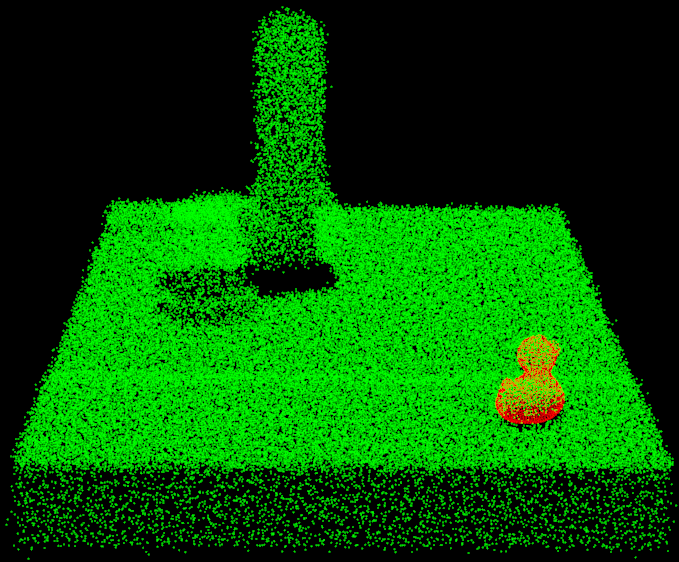
\includegraphics[width=0.3\textwidth]{figures/simulated_depth_sensor/filter/initial_scene.png}};
\node at (-6, -2.5) {(a) Input scene.};
\draw[->, thick] (-3.5,0) -- (-2.75,0);

% filtering
\node at (0, 5) {Cloud processing};
\draw[thick, dashed] (-2.5, -5.25) rectangle ++(5,10);

% spatial filter
\node[inner sep=0pt] (vertical) at (0, 4) {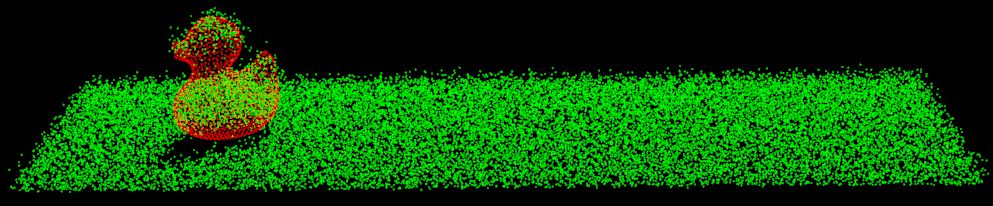
\includegraphics[width=0.3\textwidth]{figures/simulated_depth_sensor/filter/spatial_filter.png}};
\node at (0, 3.25) {(b) Spatial filter.};
\draw[->,thick] (0, 3) -- (0, 2.6);

% voxel grid
\node[inner sep=0pt] (vertical) at (0, 2) {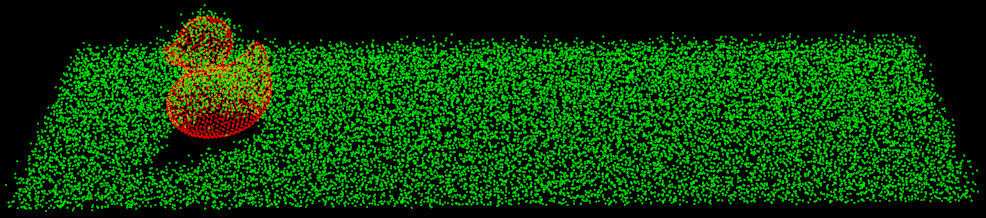
\includegraphics[width=0.3\textwidth]{figures/simulated_depth_sensor/filter/voxel_grid.png}};
\node at (0, 1.25) {(c) Voxel grid.};
\draw[->, thick] (0, 1) -- (0, 0.6);

% smoothing
\node[inner sep=0pt] (vertical) at (0, 0) {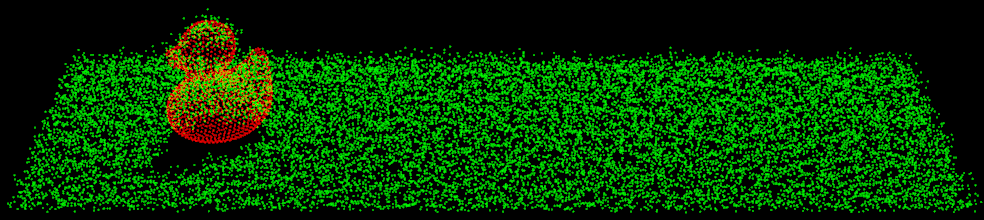
\includegraphics[width=0.3\textwidth]{figures/simulated_depth_sensor/filter/smoothing.png}};
\node at (0, -0.75) {(d) Smoothing.};
\draw[->,thick] (0, -1) -- (0, -1.4);

% planar segmentation
\node[inner sep=0pt] (vertical) at (0, -2) {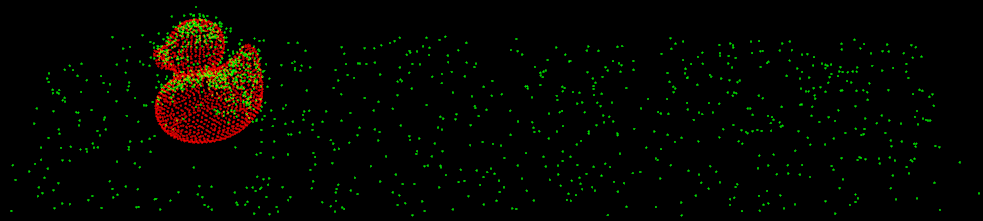
\includegraphics[width=0.3\textwidth]{figures/simulated_depth_sensor/filter/planar_segmentation.png}};
\node at (0, -2.75) {(e) Planar segmentation.};
\draw[->,thick] (0, -3) -- (0, -3.4);

% outlier removal
\node[inner sep=0pt] (vertical) at (0, -4) {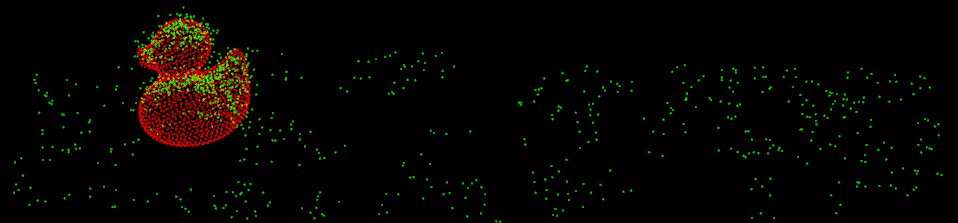
\includegraphics[width=0.3\textwidth]{figures/simulated_depth_sensor/filter/outlier_removal.png}};
\node at (0, -4.75) {(f) Outlier removal.};

% Global
\draw[->, thick, dashed] (2.75, 0) -- (3.75, 0);
\node[block] at (5, 0) {Global alignment};

\end{tikzpicture}

}

%\end{document}






